\section{Experiments}
\label{sec:experiments}

We evaluate TransitDuet on an event-driven bus microsimulation. In the main configuration, the upper policy selects rolling planned-headway adjustments that the simulator converts into planned dispatch times. The lower holding controller tracks the resulting dynamic timetable. A target-headway-only configuration is retained as an ablation.

%% ============================================================
\subsection{Experimental setup}
\label{sec:exp_setup}

\paragraph{Simulation environment.}
The simulator models a single bidirectional bus corridor with 22 stations (11 per direction) and 264 trips per service day. Passenger arrivals follow time-varying origin--destination demand matrices with stochastic per-hour demand multipliers $\mathcal{N}(1,0.15^2)$ clipped to $[0.3,2.0]$. Link travel times are log-normal with route stochasticity $\sigma_{\mathrm{route}}=1.5$ unless otherwise stated. The simulation step is one second; passenger states update every 20 seconds. The upper policy is event-driven and acts after each actual dispatch to select the planned-headway adjustment for the next same-direction trip. The lower policy acts at station arrivals.

\paragraph{Compared methods.}
The main method uses a categorical upper policy over five planned-headway adjustments from $-60$ to $+60$\,s and a categorical lower holding policy over eight holding bins from 0 to 30\,s. We compare it with the following ablations and baselines:
\begin{itemize}[leftmargin=*]
    \item Target-headway-only variant: the upper changes the lower reference headway but does not alter planned launch times.
    \item Wider-action rolling timetable: an ablation with a nine-bin upper action and 60\,s maximum holding.
    \item Continuous rolling timetable: timetable mode with a continuous upper action instead of the categorical timetable action.
    \item No-context rolling timetable: timetable mode without the lower state additions for last action, neighboring planned gaps, and station phase.
    \item Fixed-timetable SAC (holding-only SAC): a fixed rolling timetable with the same lower SAC controller, including a 360\,s reference and the best fixed headway from $\{300,330,360,390,420\}$\,s.
    \item Independent assembly: a fixed-timetable lower controller is trained first, frozen, and then paired with a trained timetable upper.
    \item Classical and RL holding baselines: Daganzo-style holding \citep{daganzo2009headway}, Xuan-style two-headway holding \citep{xuan2011dynamic}, and a same-simulator advantage-based auxiliary-reward RL proxy motivated by hierarchical RL and recent RL/MARL holding benchmarks \citep{li2019hierarchical,singh2024piper,wang2021asynchronous,wang2023robust,yu2024hierarchical,xu2025systematic,li2026graphaware}. These proxies are not claimed as exact reproductions of the original papers.
\end{itemize}

\paragraph{Metrics.}
In addition to average out-of-vehicle wait, headway CV, fleet overshoot, and the composite cost, we report average holding time, onboard passenger time, total passenger time, and dispatch lateness. We also report the variance of the planned timetable sequence and its correlation with realised headway CV.

The composite cost aggregates the three measurement components into a single evaluation scalar. It is computed as the negated upper-level reward (Eq.~\ref{eq:morl_reward}) under fixed evaluation weights $(w_{\mathrm{wait}}, w_{\mathrm{fleet}}, w_{\mathrm{cv}}) = (0.5, 0.25, 0.25)$, applied uniformly across all methods. Lower composite cost is better.

\paragraph{Training and selection.}
Each learned method is trained for 300 episodes per seed with ten seeds: 42, 123, 456, 789, 1001, 1002, 1003, 1004, 1005, and 1006. For each seed we evaluate checkpoints at episodes 49, 99, 149, 199, 249, and 299 with 20 fresh held-out episodes, and select the checkpoint with the lowest mean composite cost when checkpoint evaluation is used. The tables below report the final 30 training episodes per seed because these columns include the newly added holding, passenger-time, and timetable-feasibility diagnostics.

%% ============================================================
\subsection{Main results}
\label{sec:main_results}

\Cref{tab:main_results} reports the main comparison from the final 30 training episodes across ten seeds. Because the rolling-timetable implementation changes the action semantics, the target-headway-only configuration is reported as an ablation rather than as the main TransitDuet result.

\begin{table}[H]
\centering
\caption{Main comparison under the rolling-timetable protocol. Learned methods report mean values over ten seeds (final 30 training episodes per seed); rule-based methods report ten seeds (30 evaluation episodes per seed). Wait, onboard, and total time are in minutes; holding is in seconds. Lower is better for all metrics.}
\label{tab:main_results}
\scriptsize
\setlength{\tabcolsep}{2.2pt}
\begin{tabular}{@{}lccccccc@{}}
\toprule
Method & Wait & CV & Overshoot & Composite & Hold & Onboard & Total time \\
\midrule
TransitDuet timetable & \textbf{6.05} & 0.484 & 1.96 & \textbf{1.634} & 15.59 & \textbf{12.10} & \textbf{18.15} \\
Target-headway only & 6.58 & 0.516 & \textbf{1.93} & 1.687 & \textbf{8.47} & 12.72 & 19.30 \\
Advantage-based RL proxy & 7.23 & 0.524 & 2.03 & 1.802 & 10.22 & 12.85 & 20.08 \\
Best fixed timetable SAC (holding-only, 300\,s) & 6.90 & \textbf{0.444} & 2.77 & 1.846 & 25.69 & 13.02 & 19.92 \\
Fixed timetable SAC (holding-only, 360\,s) & 10.64 & 0.504 & 2.28 & 2.191 & 29.67 & 13.66 & 24.30 \\
Daganzo-style holding proxy & 8.86 & 0.520 & 2.36 & 2.040 & 45.15 & 13.20 & 22.06 \\
Xuan-style holding proxy & 8.49 & 0.530 & 2.47 & 2.025 & 48.33 & 13.34 & 21.83 \\
\bottomrule
\end{tabular}
\end{table}

TransitDuet achieves the lowest mean composite cost (1.634) in this comparison, 3.2\% below the target-headway-only variant (1.687) and 11.5\% below the best fixed-timetable SAC baseline (1.846). Its mean total passenger time is 18.15 minutes versus 19.30 and 19.92 minutes for these two comparators.

The table reveals a notable trade-off between headway regularity and fleet utilisation. The best fixed-timetable SAC (300\,s) achieves the lowest CV (0.444) but incurs the highest fleet overshoot among learned methods (2.77), which drives its composite cost well above TransitDuet's despite comparable waiting time. This suggests that aggressive holding for regularity can push fleet usage beyond budget constraints.

TransitDuet's mean holding time (15.59\,s) falls between the target-headway-only variant (8.47\,s) and the fixed-timetable baselines (25.69--29.67\,s). The additional holding relative to the target-headway-only variant translates into a 0.53-minute reduction in mean waiting time and a 1.15-minute reduction in total passenger time, indicating a favourable trade-off. The two classical rules apply substantially longer holding (45--48\,s) yet yield higher waiting time and total passenger time, illustrating diminishing returns from excessive holding without timetable adaptation.

%% ============================================================
\subsection{Timetable ablations}
\label{sec:ablation}

\Cref{tab:ablations} isolates the design choices in TransitDuet. The target-headway-only row tests adaptive target tuning; the fixed-timetable row isolates whether dynamic planned dispatch times add value beyond the same lower holding controller under a fixed timetable.

\begin{table}[H]
\centering
\caption{Timetable ablations. The target-headway-only row does not change planned launch times and is not treated as the main method. Lower is better for each numeric column; $\Delta$Cost is relative to the final rolling-timetable configuration.}
\label{tab:ablations}
\scriptsize
\setlength{\tabcolsep}{2.4pt}
\begin{tabular}{@{}lcccccc@{}}
\toprule
Variant & Wait & CV & Cost & Shift variation & Late & $\Delta$Cost \\
\midrule
Final rolling timetable & \textbf{6.05} & 0.484 & \textbf{1.634} & \textbf{360.3} & 25.5 & -- \\
Target-headway only & 6.58 & 0.516 & 1.687 & -- & -- & +3.2\% \\
Best fixed timetable SAC & 6.90 & \textbf{0.444} & 1.846 & 1827.6 & 38.5 & +13.0\% \\
Wider-action rolling timetable & 6.18 & 0.508 & 1.760 & 712.9 & 25.7 & +7.7\% \\
Continuous rolling timetable & 7.70 & 0.512 & 1.856 & 633.6 & \textbf{12.5} & +13.6\% \\
No-context rolling timetable & 9.45 & 0.519 & 2.048 & 706.5 & 18.3 & +25.3\% \\
Independent assembly & 7.27 & 0.512 & 1.929 & 855.3 & 34.2 & +18.1\% \\
\bottomrule
\end{tabular}
\end{table}

The planned-shift and lateness columns serve as feasibility checks for the timetable claim. A non-zero planned-shift variance confirms that the upper policy actively modifies the planned dispatch sequence, while dispatch lateness quantifies the delay between planned and actual dispatch caused by vehicle availability or fleet limits.

Among the timetable variants, the wider-action grid (+7.7\%) demonstrates that a larger action space does not guarantee improvement; the finer discretisation may introduce additional exploration difficulty without proportional benefit. The continuous variant produces the lowest dispatch lateness (12.5\,s) yet the worst composite cost among timetable variants (+13.6\%), suggesting that continuous actions complicate policy learning despite allowing smoother adjustments. Removing the lower-state context (planned-dispatch gaps, station phase, and last action) causes the largest degradation (+25.3\%), confirming that this contextual information is essential for effective holding under a dynamic timetable.

The independent-assembly result (+18.1\%) indicates that joint training contributes to the observed gains: when the lower policy cannot adapt to the rolling timetable during training, performance degrades. This supports describing TransitDuet as a jointly trained framework, although the result does not rule out that alternative coupling strategies could close the gap.

%% ============================================================
\subsection{Timetable variability and realised regularity}
\label{sec:mechanism}

For each evaluation episode, we compute the variance of planned dispatch headways and the realised dispatch-headway CV. This diagnostic tests whether variation in the planned sequence is transmitted to realised dispatch regularity.

\begin{figure}[H]
    \centering
    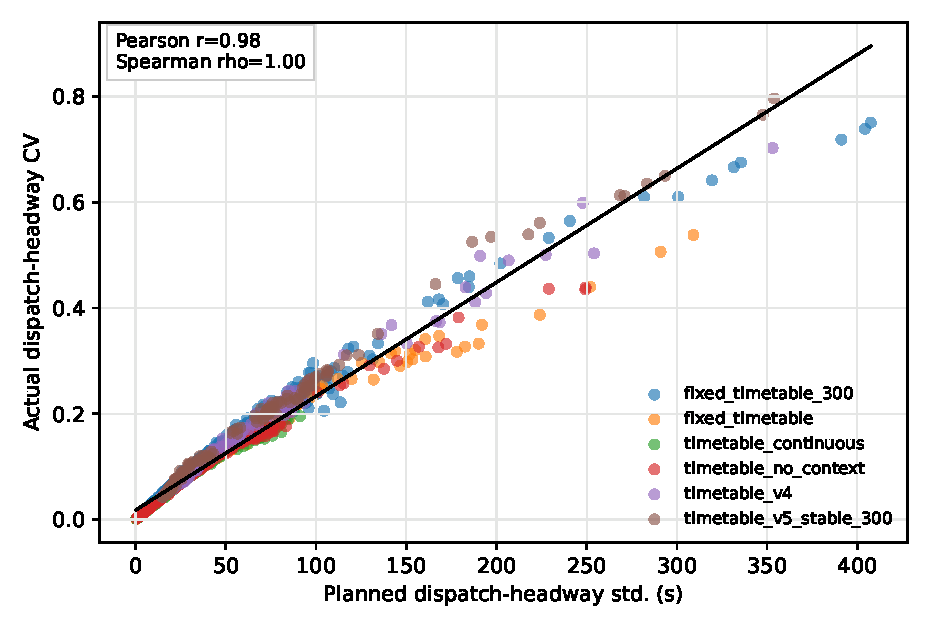
\includegraphics[width=0.62\textwidth]{figures/timetable_variance_correlation.pdf}
    \caption{Planned timetable variability versus realised dispatch-headway CV. Each point is one evaluation episode.}
    \label{fig:timetable_variance_correlation}
\end{figure}

\begin{table}[H]
\centering
\caption{Correlation between planned timetable variability and realised regularity (300 episode-level observations per method: 10 seeds $\times$ 30 final episodes).}
\label{tab:timetable_correlation}
\small
\begin{tabular}{@{}lcccc@{}}
\toprule
Method & Seeds & Observations & Pearson $r$ & Spearman $\rho$ \\
\midrule
Final rolling timetable & 10 & 300 & 0.994 & 0.981 \\
Wider-action rolling timetable & 10 & 300 & 0.990 & 0.998 \\
Continuous rolling timetable & 10 & 300 & 0.995 & 0.999 \\
No-context rolling timetable & 10 & 300 & 0.989 & 0.999 \\
Best fixed timetable SAC & 10 & 300 & 0.982 & 0.997 \\
Target-headway only & 10 & 300 & -- & -- \\
\bottomrule
\end{tabular}
\end{table}

The near-perfect correlations (Pearson $r > 0.98$ for all timetable variants) confirm that variation in the planned dispatch sequence is faithfully transmitted to realised dispatch regularity, validating the timetable channel as an effective control lever. The target-headway-only variant does not alter planned dispatch times and therefore cannot report this correlation.
